
\chapter{Modelando a Credibilidade com Programação Genética}
\label{cap::programacao_genetica}

No Capítulo~\ref{cap::metodo},
além de mostrarmos os algoritmos de classificação \textit{Naïve Bayes} e \textsc{KNN}, vimos como podemos incorporar a credibilidade nos mesmos.
Discutimos também que existem várias métricas que podem ser utilizadas para mensurar a credibilidade de um exemplo, 
embora não detalhamos essas métricas.

Nessa dissertação, modelamos a credibilidade em duas abordagens diferentes, uma levando em consideração os atributos dos exemplos e outra utilizando os seus relacionamentos. 
Em ambas, somos capazes de gerar uma grande gama de métricas que conseguem capturar a relação entre os exemplos e uma determinada classe.
Entretanto, necessitamos de uma forma de selecionar e combinar essas métricas de uma maneira robusta. Para solucionar esse problema, recorremos ao uso de Programação Genética (\textsc{PG}).

Segundo a Teoria da Evolução de Darwin, indivíduos mais adaptados ao ambiente em que se encontram têm uma chance maior de sobreviverem e se reproduzirem, passando seu material genético às gerações posteriores. Baseado nessa teoria, o método Programação Genética é adequado para evoluir uma função de credibilidade, pois possui mecanismos de busca que o torna capaz de explorar bem o imenso espaço de soluções formado pelo grande número de métricas disponíveis (\cite{Fogel00}). Além disso, \textsc{PG} é flexível o bastante para ser capaz de representar as funções que desejamos, sendo também tolerante a ruído.
%Programação Genética é um método baseado na Teoria da Evolução de Darwin que define que indivíduos mais adaptados ao ambiente em que se encontram têm uma maior chance de sobreviverem e se reproduzirem, passando seu material genético às gerações posteriores. PG é um método adequado para evoluir uma função de credibilidade, pois consegue explorar bem o imenso espaço de soluções formado pelo grande número de métricas disponíveis e é flexível o bastante para podermos representar as funções que desejamos.

Para entendermos melhor como é o funcionamento de um \textsc{PG}, utilizamos a Figura~\ref{fig::gpwf}. Ela ilustra de forma genérica os seus principais componentes.
Como podemos ver, o primeiro passo é definir um conjunto de funções e terminais para serem usados pelo \textsc{PG}.
É a partir desse conjunto de elementos que criamos nossos indivíduos.
Esses, por sua vez, são soluções candidatas para o problema que abordamos (no caso, um indivíduo é uma possível função de credibilidade).
Um conjunto de indivíduos é chamado de população e, como mostrado pelo segundo retângulo no diagrama da Figura~\ref{fig::gpwf}, a população inicial é criada aleatoriamente. 
Cada indivíduo da população é então avaliado por uma função de \textit{fitness}, que calcula a habilidade do mesmo em resolver o problema apresentado, ou seja, o quão bom aquele indivíduo é.

\begin{figure}[t]
\centering
%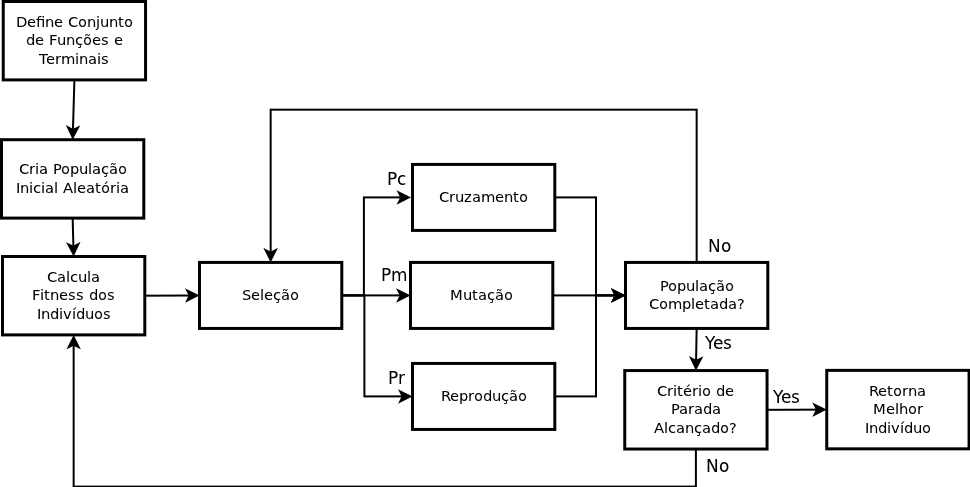
\includegraphics[width=1.0\textwidth]{figures/gpwf.png}
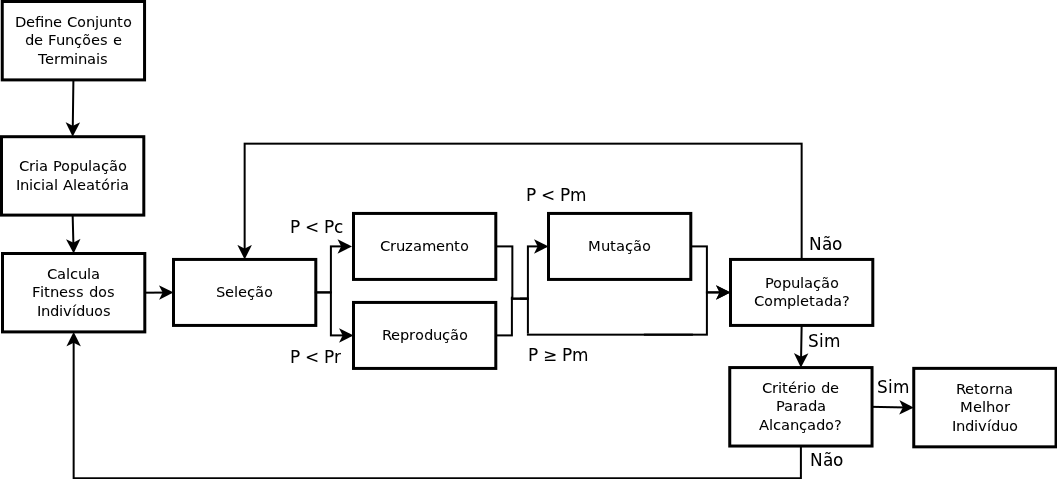
\includegraphics[width=1.1\textwidth]{figures/gpwf_new.png}
\caption{Fluxograma de um algoritmo de Programação Genética}
\label{fig::gpwf}
\end{figure}

Após avaliarmos a \textit{fitness} dos indivíduos, os melhores são selecionados e submetidos às operações genéticas de cruzamento, mutação e reprodução, com probabilidade $P_c$, $P_m$ e $P_r$, respectivamente definidas pelo usuário.
Uma forma muito usada de selecionar os indivíduos é através de torneios, nos quais tomamos aleatoriamente um número pré-definido de indivíduos da população e selecionamos aquele com maior valor da função de \textit{fitness}. Existem diversas outras variações do método de seleção (\cite{Koza92}), sendo que o importante é a utilização do conhecimento da função \textit{fitness} dos indivíduos de forma a criamos uma próxima geração mais bem preparada para resolução do problema. 

Depois de serem selecionados, os indivíduos podem passar por reprodução ou cruzamento, com probabilidades $P_r$ e $P_c$, respectivamente. 
A operação genética de reprodução simplesmente transfere o indivíduo para próxima geração, enquanto o cruzamento exige a participação de dois indivíduos que são combinados a fim de obtermos
uma prole mais adaptada na próxima geração.
Após esse processo, o indivíduo resultante da reprodução ou cruzamento pode ser submetido a mutação com uma probabilidade $P_m$.
Em geral, a mutação é uma pequena alteração em alguma parte especifica do indivíduo, alterando uma função interna ou um terminal.
Variações nas quais a operação de mutação ocorre em paralelo a de reprodução ou cruzamento também são comuns na literatura.

Esse processo de criação de indivíduos é repetido até alcançarmos um número limite do tamanho da população. Após chegarmos a esse limite, uma nova geração é iniciada. Além disso, limitar o número de gerações é uma forma muito comum de terminarmos a execução do \textsc{PG}. Outras formas seriam chegar à um variação arbitrariamente pequena de melhoria ou algum indivíduo conseguir alcançar um valor de \textit{fitness} pré-definido. Por fim, o \textsc{PG} retorna o melhor indivíduo evoluído.

%Depois de serem selecionados, os indivíduos podem sofrer alguma alteração genética através das operações de mutação e cruzamento ou podem ser transferidos diretamente para a próxima geração, através da reprodução. 
%a operação de mutação, uma parte do indivíduo selecionado é aleatoriamente alterada, buscando obter uma melhoria da \textit{fitness} na próxima geração.
%or sua vez, a operação de cruzamento exige a participação de dois indivíduos que são combinados a fim de obtermos uma prole mais adaptada na próxima geração.
%o modo como está mostrado na Figura~\ref{fig::gpwf}, somente uma dessas três operações é realizada em cada indivíduo selecionado, entretanto é comum também implementações em que é aplicada a probabilidade de mutação para todos os indivíduos, logo após uma nova prole ser gerada pelo cruzamento ou reprodução.

Repare que todo o processo exposto na Figura~\ref{fig::gpwf} é \textit{independente} da aplicação na qual o \textsc{PG} é utilizado. 
Entretanto, três importantes componentes devem ser instanciados dependendo do contexto no qual trabalhamos. Eles são:
\begin{enumerate}
\item A representação dos indivíduos, que inclue as funções do \textsc{PG} e terminais relevantes a aplicação, e são abordados na Seção~\ref{subsec::individuos}, 
\item Os operadores genéticos, descritos na Seção~\ref{subsec::operadoresgeneticos},
\item A função de \textit{fitness} detalhada na Seção~\ref{subsec::fitness}.
\end{enumerate}
Além disso, pelo fato de termos uma vasta gama de terminais e queremos explicar um por um deles, separamos as Seções~\ref{sec::pg_cred_baseada_conteudo} e \ref{sec::pg_cred_baseada_grafos} para explicarmos com detalhes as métricas baseadas em atributos e em relacionamentos, respectivamente.

\section{Indivíduos}
\label{subsec::individuos}

Uma parte essencial da construção de um \textsc{PG} é definir os indivíduos que compõem a população do mesmo.
Para isso, temos que definir três aspectos primordiais: o que um indivíduo representa, quais são suas funções internas e quais são os seus terminais. Independente de quais são as funções internas e terminais escolhidos, o propósito de um indivíduo no \textsc{PG} modelado é representar uma função de credibilidade que, a não ser que seja dito o contrário, relaciona um exemplo de teste, seja por seus atributos ou relacionamentos, a uma classe, retornando um valor real. 

Como já discutido nas Seções~\ref{subsubsec::nbcredatributos} e \ref{subsubsec::nbcredgrafos} para o \textit{Naïve Bayes} e Seções~\ref{subsubsec::knncredatributos} e \ref{subsubsec::knncredgrafos} para o \textsc{KNN}, modelamos duas funções de credibilidade diferentes, uma baseada nos atributos dos exemplos e outra baseada nos relacionamentos dos mesmos.
Ambas, entretanto, compartilham o mesmo conjunto de funções internas, porém os terminais utilizados são diferentes para cada caso. As funções internas são utilizadas para que haja uma interação entre os terminais.
Como usual para um \textsc{PG} que evolui uma função matemática numérica, as funções internas do \textsc{PG} consistem de funções matemáticas conhecidas, como a multiplicação, divisão, soma, entre outros que estão mostradas na Tabela~\ref{table::funcoespg}. 
Observe que modificamos as funções de subtração, divisão e logaritmo.
Tanto a divisão por zero, quanto o logaritmo de números negativos não são matematicamente definidos, portanto explicitamente tratamos esses casos retornando zero. Além disso, não queremos ter uma função de credibilidade negativa, portanto evitamos que a subtração e o logaritmo retornem números negativos.

\begin{table}[ht*]
\centering
\begin{tabular}{|c|c|}
\toprule
    \textbf{Função Interna} & \textbf{Explicação} \\
\midrule
    $+(a,b)$           & Soma $a$ com $b$. \tabularnewline \hline
    $-(a,b)$           & Subtrai $b$ de $a$, porém retorna 0 se $b$ for maior que $a$.\tabularnewline \hline
    $\times(a,b) $     & Multiplica $a$ com $b$. \tabularnewline \hline
    $\%(a,b)$          & Divide $a$ por $b$, porém retorna 0 se $b$ for 0. \tabularnewline \hline
    $\text{Pow}(a,b)$  & Eleva $a$ a potência de $b$. \tabularnewline \hline 
    $\log(a,b) $       & Logaritmo de $a$ na base $b$, retorna 0 se $a$ ou $b$ forem menores que 1. \tabularnewline
\bottomrule
\end{tabular}
\caption{XXXXXXXXXXXXX.}
\label{table::funcoespg}
\end{table}

Pelo fato de termos um grande número de terminais definidos, reservamos as Seções~\ref{sec::pg_cred_baseada_conteudo} e~\ref{sec::pg_cred_baseada_grafos} exclusivamente para descrevermos aqueles relacionados ao atributos dos exemplos e em mensurar os relacionamentos entre os exemplos, respectivamente. Na Figuras~\ref{fig::gps1} e~\ref{fig::gps2} temos ao todo cinco exemplos de funções de credibilidades que poderiam ser geradas pelo \textsc{PG}, as três da primeira figura ilustram funções de credibilidade baseadas em atributos e as demais são baseadas em relacionamentos entre os exemplos. As cores nas mesmas são usadas apenas para auxiliar na explicação das operações genéticas de mutação e cruzamento na seção a seguir.

\begin{figure}[ht]
\centering
\subfloat[Individuo 1:\newline \hspace*{6mm}$\textsc{GINI}(x)^{\textsc{CC}(x,c)}$]{
    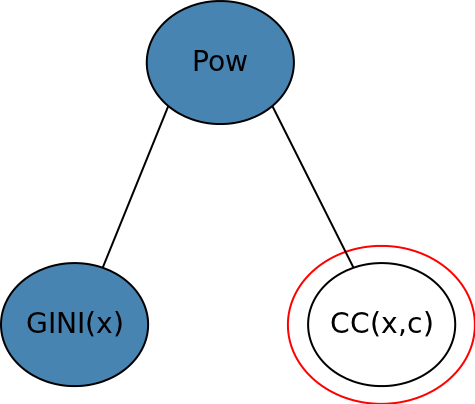
\includegraphics[width=0.25\textwidth]{figures/gp1c.png}
}
\subfloat[Individuo 2:\newline \hspace*{4mm} $(\textsc{AM}(x,c) + \textsc{P}(x|c)) \% (\textsc{IG}(x,c))$]{
    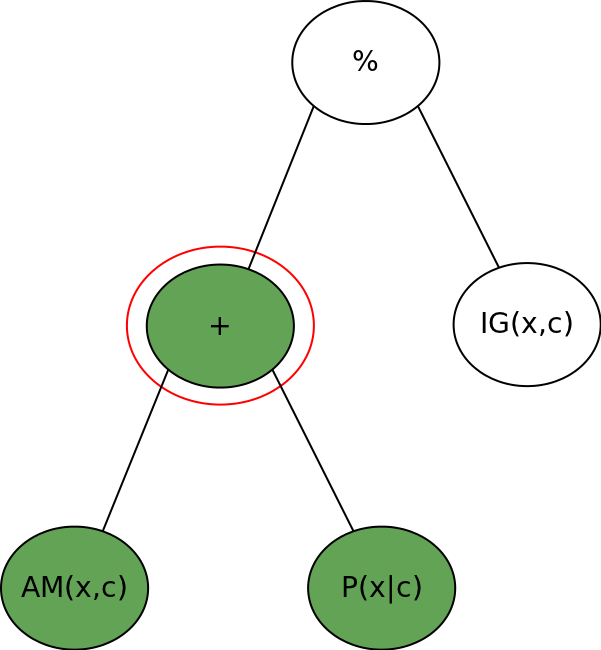
\includegraphics[width=0.33\textwidth]{figures/gp2c.png}
}
\subfloat[Individual 3:\newline \hspace*{4mm} $\textsc{GINI}(x)^{(\textsc{AM}(x,c)\ + \ \textsc{P}(x|c))}$]{
    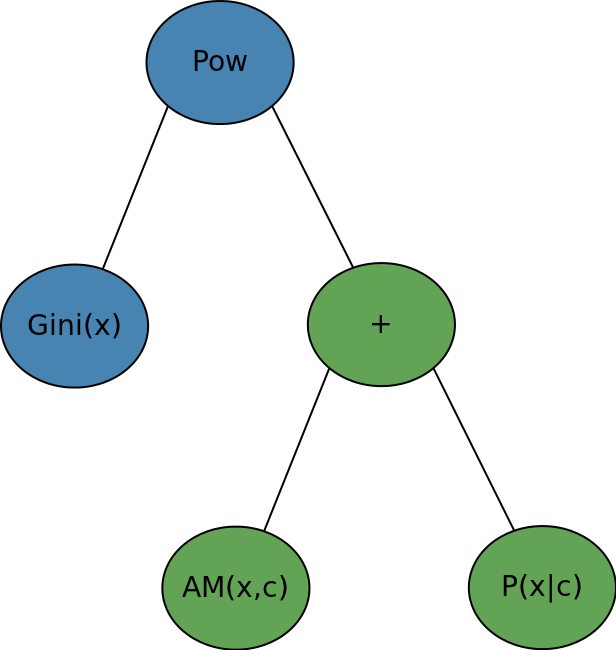
\includegraphics[width=0.33\textwidth]{figures/gp3c.png}
}
\caption{Três possíveis indivíduos gerados para representar uma função de credibilidade de atributos.}
\label{fig::gps1}
\end{figure}


\begin{figure}[ht]
\centering
\subfloat[Individuo 1:\newline \hspace*{6mm}$\textsc{Bib}(X,c) - {\textsc{Hub}(x,c)}$]{
%\subfloat[Individuo 1:$\textsc{Bib}(X,c) - {\textsc{Hub}(x,c)}$]{
    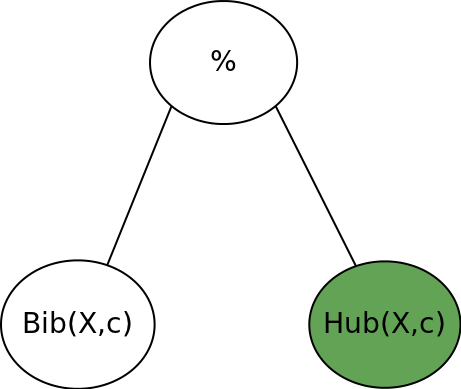
\includegraphics[width=0.30\textwidth]{figures/gp1c_grafos.png}
}
\subfloat[Individuo 2:\newline \hspace*{5mm} $\textsc{Bib}(X,c) - \textsc{PR}(X,c) $]{
    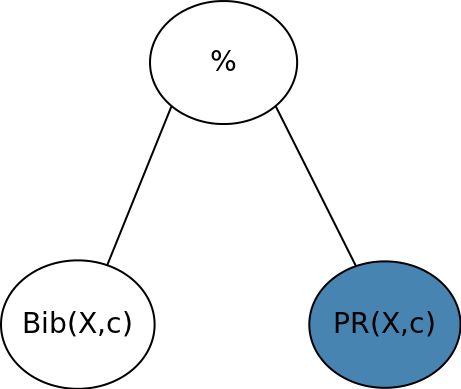
\includegraphics[width=0.30\textwidth]{figures/gp2c_grafos.png}
}
\caption{Dois possíveis indivíduos gerados para representar uma função de credibilidade para relacionamentos.}
\label{fig::gps2}
\end{figure}

\section{Operadores Genéticos}
\label{subsec::operadoresgeneticos}

Em nosso trabalho, utilizamos três operadores genéticos na geração dos indivíduos, como mostrado na Figura~\ref{fig::gpwf}. 
Primeiramente, os indivíduos podem ser submetidos as operações de cruzamento ou reprodução. 
%Para o primeiro caso, sorteamos dois indivíduos, para reprodução, somente um. 
Os indivíduos usados nessas operações são selecionados por meio de um torneio, onde escolhemos aleatoriamente $T$ indivíduos da população atual (parâmetro configurado pelo usuário) e dizemos que aquele com maior \textit{fitness} é o ganhador do torneio. 
%Primeiramente, como exibido, os indivíduos podem ser submetidos as operações de cruzamento, mutação ou reprodução. 
%Para o primeiro caso, sorteamos dois indivíduos, para mutação ou reprodução, somente um. 
%Os indivíduos são selecionados por meio de um torneio, onde escolhemos aleatoriamente $T$ indivíduos da população atual e dizemos que aquele com maior \textit{fitness} é o ganhador do torneio.

A operação de reprodução é a mais simples, e insere o indivíduo ganhador do torneio na próxima geração sem realizar nenhuma modificação. Já na operação de cruzamento, realizarmos dois torneios, selecionando dois indivíduos. Depois disso, escolhemos aleatoriamente um ponto em cada um dos dois indivíduos selecionados e geramos dois novos indivíduos contendo partes de ambos os pais. A Figura~\ref{fig::gps1} ilustra esse processo. 
Os indivíduos 1 e 2 são selecionados utilizando dois torneios distintos, e neles são escolhidos dois pontos para que ocorra a operação de cruzamento genético. 
No indivíduo 1, o ponto de troca escolhido foi a métrica 
\textsc{CC(x,c)} 
e no indivíduo 2, a função ``+'', ambos em destaque na Figura~\ref{fig::gps1}.
Por fim, trocamos a métrica \textsc{CC(x,c)} pela subárvore do nó selecionado indivíduo 2, gerando o indivíduo 3. 
Note que também é gerado um indivíduo 4 (não mostrado na figura) representando a função de credibilidade \textsc{Cred(x,c) = CC(x,c) \% IG(x,c)}. 

Finalmente, a prole resultante da reprodução ou cruzamento, pode ser submetida a operação de mutação. Utilizamos a mutação de ponto, na qual o indivíduo tem uma probabilidade $P_m$ de ter um ponto selecionado para a substituição de um terminal ou função por outro aleatório.
Na Figura~\ref{fig::gps2}, vemos uma mutação ocorrendo no indivíduo 1, gerando o indivíduo 2. Note que a métrica \textsc{Hub} foi substituída pela métrica \textit{PageRank} (\textsc{PR}).

%---------------------------------------------------------------------------------
%---------------------------------------------------------------------------------
%---------------------------------------------------------------------------------
%---------------------------------------------------------------------------------

\section{\textit{Fitness}}
\label{subsec::fitness}

Necessitamos de um modo de avaliar os indivíduos da população a fim de sabermos quais são aqueles mais aptos a sobreviverem para a próxima geração. 
Para tanto, utilizamos a chamada função de \textit{fitness}. 
Em nosso caso, estamos criando funções de credibilidade que serão usadas para que um classificador possa criar modelos de classificação mais aprimorados.
Dessa forma, nossa função de \textit{fitness} tem que estar atrelada a uma forma de avaliar o quanto o classificador melhorou ou piorou ao incorporarmos a ele um função de crebilidade gerada.
Uma métrica muito utilizada na literatura para avaliação de classificadores é a $F_1$ e, por isso, decidimos por utilizá-la.
% --> continuar depois..... tenho auqe falar que podemos usar as metricas ja usadas para ver se um metodo de classificacao eh bom, como F1.
%Portanto, podemos utilizar as métricas de avaliação de classificadores para que possamos 
No Algoritmo~\ref{alg::fitness}, descrevemos o processo usado para calcular a \textit{fitness} de um individuo levando em consideração funções evoluídas tanto para atributos quanto para relacionamentos.

\algrenewcommand\algorithmicforall{\textbf{Para Cada}}
\algrenewcommand\algorithmicdo{\textbf{Faça}}
\algrenewcommand\algorithmicfunction{\textbf{Função}}
\algrenewcommand\algorithmicif{\textbf{Se}}
\algrenewcommand{\algorithmicreturn}{\textbf{retorna}} %% nao sei pq nao funciona, pesquisar depois

\begin{algorithm}
\centering
\caption{Calula Fitness.}
\label{alg::fitness}
\begin{algorithmic}[h]
{
%\scriptsize
\Function{CalculaFitness}{$individuo$}
  \State  
  \State \textit{Credibilidade dos atributos:}
  \If{Utilizando Credibilidade Baseada em Atributos}
  \ForAll{$x \in \mathbb{A}$}
    \ForAll{$c \in \mathbb{C}$}
      \State $f_a(x,c) \gets eval(individuo_{attrs}, x, c)$
    \EndFor
  \EndFor
  \EndIf
  \State
  
  \State \textit{Credibilidade dos relacionamentos:}
  \If{Utilizando Credibilidade Baseada em Relacionamentos}
  \ForAll{$r \in \mathbb{R}$}
    \ForAll{$e \in \mathbb{E}$}
        \ForAll{$c \in \mathbb{C}$}
            \State $f_r(r,d,c) \gets eval(r,individuo_{rel}, d, c)$
        \EndFor
    \EndFor
  \EndFor
  \EndIf
  \State
  \State \textit{Avaliação da Fitness:}
  \State fitness $\gets$ \textsc{F$_1$}(\textsc{Classifier}$(\mathbb{T}, \mathbb{E}, \mathbb{C}, f_x, f_r)$)
  \State \textbf{return} fitness
\EndFunction
}
\end{algorithmic}
\end{algorithm}


Começamos o Algoritmo~\ref{alg::fitness} com a formação do mapeamento $f_a$, formado pela aplicação da função de credibilidade que o indivíduo representa a cada par de atributos e classes.
Logo depois, calculamos a credibilidade de cada relacionamento no conjunto $\mathbb{R}$ de relacionamentos, usando o conjunto $\mathbb{E}$ de exemplos de treinamento em um mapa $f_r$.
Por fim, o classificador recebe o conjunto $\mathbb{T}$ de exemplos de teste, o conjunto $\mathbb{E}$ de exemplos de treinamento, o conjunto $\mathbb{C}$ de classes e os valores mapeados para as funções $f_a$ e $f_r$ de credibilidade de atributos e relacionamentos, respectivamente, retornando para cada exemplo de $\mathbb{T}$ uma possível classe de $\mathbb{C}$.
Assim, podemos calcular qual o valor da métrica chamada \textit{$F_1$} baseada nos resultados do classificador utilizado. 

Para explicar a métrica $F_1$, utilizamos a Tabela~\ref{table::confusao}. Nela, temos um cenário simplificado no qual duas classes são possíveis para uma instância de teste, + e -, e as quatro situações podem ser geradas, VP, FP, FN ou VN. Dessa forma, VP é a situação na qual o exemplo de teste pertence a classe + e é classificado corretamente (verdadeiro positivo), FP ocorre quando o exemplo é da classe - e é classificado como + (falso positivo), FN ocorre nas vezes quando o exemplo pertence a classe + e classificado como - (falso negativo) e, finalmente, VN é quando classificamos o exemplo como - e realmente pertence a - (verdadeiro negativo).


\begin{table}[ht*]
\centering
\begin{tabular}{|c|c|c|}
\toprule
       &    \textbf{Pertence a classe +} & \textbf{Pertence a classe -} \\
\midrule
    \textbf{Classificado como +}  & VP & FP \tabularnewline \hline
    \textbf{Classificado como -}  & FN & VN \tabularnewline
\bottomrule
\end{tabular}
\caption{Matriz de confusão usada para exemplificar as métricas de precisão e revocação.}
\label{table::confusao}
\end{table}

A partir dos conceitos de VP, FP, FN e VN, podemos definir duas importantes métricas comumente utilizadas na literatura, precisão e revocação. A precisão \textsc{P} é definida como:
\begin{equation}
\textsc{P} = \frac{VP}{(VP+FN)} = \frac{\# \text{de exemplos da classe c corretamente classificados como classe c}} {\# \: \text{ total de exemplos classificados como classe c}} \\,
\end{equation}
e a revocação \textsc{R} como sendo:
\begin{equation}
\textsc{R} = \frac{VP}{(VP+FP)} = \frac{\# \: \text{de exemplos da classes c corretamente classificados como classe c}}{\# \: \text{de exemplos existentes na classe c}}.
\end{equation}
Dessa forma, a precisão calcula o quanto um classificador acerta em uma determinada classe e a revocação mede o quanto o classificador é bom em achar os exemplos pertencentes àquela classe.
Ambas métricas são bastante importantes e a média harmônica delas é utilizada para formar a medida chamada $F_1$:
\begin{equation}
\text{F}_1 = \frac{2 \cdot P \cdot R}{(P + R)}.
\end{equation}

Existem ainda duas formas derivadas da $F_1$, nomeadas \textit{micro-$F_1$} e \textit{macro-$F_1$}. A primeira, \textit{micro-$F_1$}, leva em consideração a precisão e a revocação do classificador como um todo. 
Portanto, o componente VP da Tabela~\ref{table::confusao} usado na \textit{micro-$F_1$} é representado pelo número de exemplos corretamente classificados, independente de qual classe eles pertencem.
Por sua vez, a \textit{macro-$F_1$} realiza a média da $F_1$ calculada individualmente para cada uma das classes. 

Dada a forma como são enunciadas, a \textit{macro-$F_1$} e \textit{micro-$F_1$} tendem a se diferenciar se a base de dados tiver classes desbalanceadas. Em geral, uma exemplo pertencente a uma classe pouco popular é mais difícil de ser classificado que um outro pertencente a uma classe muito popular. Portanto, se estivermos analisando uma base de dados desbalanceada, a \textit{macro-$F_1$} tenderá a ter um valor menor que a \textit{micro-$F_1$}, pois a primeira é prejudicada pelas classes mais raras. 

%A \textit{$F_1$} é uma métrica amplamente utilizada por representar um compromisso interessante entre a precisão e a revocação, outras duas importante métricas. 
%A precisão ($\textsc{P}$) calcula, para uma classe específica, o quanto o classificador acerta entre todos os exemplos que ele classificou para aquela classe: 
%\begin{equation}
%\textsc{P(c)} = \frac{\# \text{de exemplos da classe c corretamente classificados como classe c}} {\# \: \text{ total de exemplos classificados como classe c}} \\,
%\end{equation}
%logo determinamos o quão bom o classificador é em avaliar exemplos de uma classe específica. 
%Por sua vez, a revocação (\textsc{R}) calcula, para uma classe, o quanto foi corretamente classificado entre o que deveria ter sido classificado para classe em questão:
%\begin{equation}
%\textsc{R(c)} = \frac{\# \: \text{de exemplos da classes c corretamente classificados como classe c}}{\# \: \text{de exemplos existentes na classe c}},                      
%\end{equation}
%logo, calculamos o quão bom o classificador é para achar exemplos de uma dada classe. 
%Por fim, a \textit{$F_1$} é a média harmónica entre a precisão e a revocação:
%\begin{equation}
%\text{F}_1(c) = \frac{2 \cdot P(c) \cdot R(c)}{(P(c) + R(c))}.
%\end{equation}

%A partir da $F_1$ podemos calcular as métricas \textit{macro-$F_1$} e \textit{micro-$F_1$}. 

%Já a \textit{micro-$F_1$} calcula a precisão e revocação de toda a coleção de uma so vez.
%A \textit{macro-$F_1$} leva em consideração a $F_1$ de cada uma das classes e depois calcula a média das mesmas. 


%sem levar em considerar o cálculo classe a classe, portanto usamos a precisão e revocação considerando o sistema como um todo.
Por ser uma métrica amplamente mais utilizada na literatura, optamos por utilizar a \textit{micro-$F_1$} como função de \textit{fitness}. Porém sempre medimos e reportamos a \textit{macro-$F_1$}. Mostramos os resultados dos vários experimentos com \textit{micro} e \textit{macro-$F_1$}, além de uma combinação de ambas no Capítulo~\ref{cap::experimentos}.

%\begin{equation}
%\text{MacroF}_1 = \frac{\sum\limits_{c \in \mathbb{C}} F_1(c) } { |\mathbb{C}| },
%\end{equation}


\section{Credibilidade Baseada nos Atributos}
\label{sec::pg_cred_baseada_conteudo}

Nessa seção apresentamos várias métricas utilizadas na construção dos indivíduos usados pelo Programa Genético. Elas foram modeladas diferentemente para os casos nos quais os atributos são textuais ou categóricos, sendo que a modelagem para atributos numéricos foi deixada como trabalho futuro. 

Em suma, algumas métricas são muito atreladas a classificação de documentos, em especial aquelas que realizam cálculos baseados na frequência de termos e documentos. 
Entretanto, muitas são genéricas o suficiente para serem utilizadas em qualquer contexto de classificação baseada em atributos.
Dessa forma, na Seção~\ref{subsec::pg_metricas_conteudo_textual} mostramos as métricas que foram modeladas única e exclusivamente para serem utilizadas na tarefa de classificação de documentos  e na Seção~\ref{subsec::pg_metricas_conteudo} temos as métricas que foram estendidas e estão sendo usadas também para a classificação categórica.

\subsection{Métricas Modeladas Exclusivamente Para Atributos Textuais.}
\label{subsec::pg_metricas_conteudo_textual}

As métricas usadas para atributos textuais consistem em algumas variantes do \textsc{TFIDF}, métrica mais difundida entre as apresentadas. Na tabela~\ref{table::metricas_textuais} estão concentradas algumas expressões amplamente utilizadas nas métricas aqui listadas.

\begin{table}[ht*]
\centering
\begin{tabular}{|c|c|}
\toprule
    \textbf{Expressão} & \textbf{Explicação} \\
\midrule
    $N$           & Número de documentos na base de treinamento. \tabularnewline \hline
    $M$           & Número de classes da coleção. \tabularnewline \hline
    $D$           & Número de termos da coleção. \tabularnewline \hline
    $DF_{t_i} $   & Número de documentos do conjunto do treino que contém o termo $t_i$. \tabularnewline \hline
    $DF_{t_ic_j}$ & Número de documentos do treino com o termo $t_i$ e pertencentes a classe $c_j$. \tabularnewline \hline
    $CF_{t_i}$    & Número de classes em que o termo $t_i$ ocorre. \tabularnewline \hline 
    $F_{t_i}$     & Número de vezes que o termo $t_i$ aparece nos documentos de treinamento. \tabularnewline \hline
    $F_{t_ic_j}$  & Número de vezes que o termo $t_i$ aparece em documentos da classe $c_j$ no treino. \tabularnewline 
\bottomrule
\end{tabular}
\caption{Explicação das principais expressões utilizadas para definição das métricas para atributos textuais.}
\label{table::metricas_textuais}
\end{table}


%%%%%%%%%%%%%%%%%%%-------------------------------------------------------%%%%%%%%%%%%%%%%%%%%%%%%%%%%%%%%%%%%%%%%
\subsubsection{Frequência do Termo} %(TF)}
\label{subsubsection::sumtf}

A frequência de um termo (\textsc{TF} da expressão em inglês, \textit{Term Frequency}) é simplesmente o número de vezes que um termo aparece na coleção de treinamento. Utilizamos o logaritmo desse valor como um fator normalizador, para evitar que termos muito frequentes dominem a função de credibilidade:
\begin{equation}\label{eqn::sumtf}
   \textsc{TF}(t_i) = 1.0 + \log{ ( F_{t_i} ) }.
\end{equation}

Temos que $TF(t_i)$ é a primeira e uma das muitas métricas que são chamadas de métricas globais. Essa denominação provêm de trabalhos como o de \cite{Lan05} ou \cite{Liu09}, nos quais métricas que não utilizam a informação da classe são vistas como globais por terem o mesmo valor para todas as possíveis classes. Em geral, métricas que calculam máximo são globais, ver Seções~\ref{subsubsection::maxctd},~\ref{subsubsection::maxdom}, entre outras muitas.

%%%%%%%%%%%%%%%%%%%-------------------------------------------------------%%%%%%%%%%%%%%%%%%%%%%%%%%%%%%%%%%%%%%%%
\subsubsection{Frequência do Termo por Classe} % (\textsc{TFClasse})}
\label{subsubsection::tf}

A frequência de um termo em uma classe, \textsc{TFClasse}, segue o mesmo padrão utilizado pela métrica \textsc{TF}, porém dessa vez contamos apenas os termos que aparecem em uma dada classe $c_j$:
\begin{equation}\label{eqn::tf}
  \textsc{TFClasse}(t_i, c_j) = 1.0 + \log{ ( F_{t_ic_j} ) }.
\end{equation}


%%%%%%%%%%%%%%%%%%%-------------------------------------------------------%%%%%%%%%%%%%%%%%%%%%%%%%%%%%%%%%%%%%%%%
\subsubsection{Frequência dos Documentos por Termo}% (DF)}
\label{subsubsection::df}

A métrica \textsc{DF}, do inglês, \textit{Document Frequency}, procura analisar a importância de um termo em relação ao número de documentos em que o mesmo aparece:
\begin{equation}\label{eqn::df}
  \textsc{DF}(t_i) = 1.0 + \log{ ( DF_{t_i} ) }.
\end{equation}


%%%%%%%%%%%%%%%%%%%-------------------------------------------------------%%%%%%%%%%%%%%%%%%%%%%%%%%%%%%%%%%%%%%%%

\subsubsection{Frequência de Documentos por Termo-Classe}% (DFClasse)}
\label{subsubsection::sumdf}

A métrica \textsc{DFClasse} avalia o número de documentos que um termo aparece em relação a uma classe específica, tentando capturar a importância de um termo para uma classe em relação ao número de documentos onde aquele termo está presente:
\begin{equation}\label{eqn::sumtf}
 \textsc{DFClasse}(t_i,c_j) = 1.0 + \log{ ( DF_{t_ic_j} ) }.
\end{equation}


%%%%%%%%%%%%%%%%%%%-------------------------------------------------------%%%%%%%%%%%%%%%%%%%%%%%%%%%%%%%%%%%%%%%%
\subsubsection{Inverso da Frequência de Documentos}% (\textsc{IDF})}
\label{subsubsection::idf}

O Inverso da Frequência de Documentos, \textsc{IDF} do inglês \textit{Inverse Document Frequency}, é uma métrica que avalia a popularidade de um determinado termo em um conjunto de documentos. Temos que quanto mais popular é um termo ao longo dos documentos de uma coleção, pior é sua capacidade de discriminação, logo:
\begin{equation}\label{eqn::tficf}
 \textsc{IDF}(t_i) = \log( \frac{|N|} {DF_{t_i}} ).
\end{equation}

%%%%%%%%%%%%%%%%%%%-------------------------------------------------------%%%%%%%%%%%%%%%%%%%%%%%%%%%%%%%%%%%%%%%%

\subsubsection{Inverso da Frequência de Documentos por Classe}% (\textsc{IDFClasse})}
\label{subsubsection::idf}

O Inverso da Frequência de Documentos por classe, \textsc{IDFClasse} é uma versão do \textsc{IDF} em que selecionamos somente documentos de uma dada classe:
\begin{equation}\label{eqn::tficf}
 \textsc{IDFClasse}(t_i,c_j) = \log( \frac{DF_{c_j}} {DF_{t_ic_j} }).
\end{equation}


%%%%%%%%%%%%%%%%%%%-------------------------------------------------------%%%%%%%%%%%%%%%%%%%%%%%%%%%%%%%%%%%%%%%%

\subsubsection{Frequência do Termo Inverso da Frequência de Documentos}% (\textsc{TFIDF})}
\label{subsubsection::tfidf}

Uma das métricas de pesos para atributos em classificação de documentos mais populares na literatura é o \textsc{TFIDF} (do inglês, \textit{Term Frequency Inversed Document Frequency} (\cite{Salton88}). O \textsc{TFIDF} combina a frequência de um termo (\textit{Term Frequency}) que assume que múltiplas aparições de um termo em um documento são mais importantes que aparições únicas com o inverso da frequência de um documento (\textit{Inverded Document Frequency}) que diz que termos raros são de maior poder discriminativo que termos muito frequentes. Em síntese, a fórmula de \textsc{TFIDF} é:
\begin{equation}\label{eqn::tficf}
 \textsc{TFIDF}(t_i, c_j) =  F_{t_ic_j} \cdot \log( \frac{|N|} {DF_{t_i}} ).
\end{equation}

%%%%%%%%%%%%%%%%%%%-------------------------------------------------------%%%%%%%%%%%%%%%%%%%%%%%%%%%%%%%%%%%%%%%%
\subsubsection{Frequência do Termo Inverso da Frequência da Classe}% (TFICF)}
\label{subsubsection::tficf}

O \textsc{TFICF} (do inglês, \textit{Term Frequency Inversed Class Frequency}) é uma variação do \textsc{TFIDF}. Novamente, \textsc{TF} se refere a quanto importante é um termo em uma classe, pois trata-se de sua frequência. Por sua vez, \textsc{ICF} é usado para que termos que aparecem em poucas classes tenham maior importância.
Como é possível observar, uma desvantagem do \textsc{ICF} é que um termo que aparecesse em todos os documentos de uma determinada classe e em um único documento de cada uma das outras teria um o mesmo peso que um outro que fosse igualmente distribuído entre todas as classes. 
Como mostrado por~\cite{ChihHow04}, a fórmula para \textsc{TFICF} é:
\begin{equation}\label{eqn::tficf}
 \textsc{TFICF}(t_i, c_j) = N_{t_ic_j} \cdot \log( \frac{M}{CF_{t_i}} ).
\end{equation}

%%%%%%%%%%%%%%%%%%%-------------------------------------------------------%%%%%%%%%%%%%%%%%%%%%%%%%%%%%%%%%%%%%%%%
\subsubsection{\textit{Category Term Description}}
\label{subsubsection::ctd}

Definido por~\cite{ChihHow04}, \textit{Category Term Description} é uma métrica de seleção de atributos para classificação textual baseada em \textsc{TFIDF} (Seção~\ref{subsubsection::tfidf}) e \textsc{TFICF} (Seção~\ref{subsubsection::tficf}). How et al. propõe uma melhoria ao TDICF, tentando adicionar o fato que termos que aparecem em poucos documentos devem ter maior importância que os termos mais populares, pois tem maior poder discriminativo, logo:

\begin{equation}\label{eqn::cdt}
 \textsc{CDT}(t_i, c_j) = \textsc{TFClass}(t_i, c_j) \cdot \textsc{ICF}(t_i, c_j) \cdot \textsc{IDF}(t_i)
\end{equation}

\subsubsection{Máximo \textit{Category Term Description}}
\label{subsubsection::maxctd}
Calculamos o valor máximo de \textsc{CTD} para todas as classes e utilizamos esse valor como uma métrica discriminatória global que relacionará mais fortemente os termos com as classes nas quais o \textsc{CTD} é máximo. Logo, usamos:

\begin{equation}\label{eqn::maxdom}
 \textsc{MaxCTD}(t_i) = \textsc{CTD}(t_i,c_j) \; \; | \;\; \textsc{CTD}(t_i, c_j) > \textsc{CTD}(t_i, c_k), \; \forall\ c_k\ \in\ \mathbb{C}
\end{equation}

%%%%%%%%%%%%%%%%%%%-------------------------------------------------------%%%%%%%%%%%%%%%%%%%%%%%%%%%%%%%%%%%%%%%%
\subsubsection{Dominância}
\label{subsubsection::dom}

Dominância é uma métrica originalmente proposta em~\cite{Zaiane02}.
%e utilizada mais recentemente no trabalho de~\cite{Rocha08} para criação do que foi chamado de janela temporal de um documento. Em suma,
Utilizado exclusivamente em classificação textual, o método normaliza a frequência de um documento em uma classe por todas as classes existentes, logo:
\begin{equation}\label{eqn::dom}
 \textsc{Dom}(t_i, c_j) = \frac{ DF_{t_ic_j} } { \sum\limits_{c_k \in \mathbb{C}} DF_{t_ic_k} } 
\end{equation}

%\subsubsection{MaxTFIDF}
%\label{subsubsection::maxtfidf}
%\subsubsection{MaxTFICF} 
%\label{subsubsection::maxtficf}

\subsubsection{Máxima Dominância}
\label{subsubsection::maxdom}
A máxima dominância é uma métrica extrapolada da Dominância (Seção~\ref{subsubsection::dom}). Aqui trabalhamos somente em estipular a dominância global de um termo e consideramos que ela é o valor máximo entre todas as possíveis classes. Logo,

\begin{equation}\label{eqn::maxdom}
 \textsc{MaxDom}(t_i) = \textsc{Dom}(t_i,c_j) \; \; | \;\; \textsc{Dom}(t_i, c_j) > \textsc{Dom}(t_i, c_k), \; \forall\ c_k\ \in\ \mathbb{C}
\end{equation}

%

\subsection{Métricas Modeladas Para Atributos Textuais e Categóricos.}
\label{subsec::pg_metricas_conteudo}


Todas as métricas apresentadas nessa seção foram utilizadas para geração de funções de credibilidade que tratam tanto atributos textuais quanto categóricos. 
Elas são inspiradas em probabilidades que podem ser facilmente calculadas dos exemplos contidos no conjunto de treinamento. 
Destacamos que a probabilidade condicional $P(x_i|c_j)$ como a principal métrica, pois as demais, complexas ou não, são derivações dessa.

Pretendemos através da Tabela~\ref{table::metricas_textuais_categoricos} mostrar as definições utilizadas para definição dos atributos categórico, lembrando que quando se trata de um problema de classificação de texto deve-se recorrer a Tabela~\ref{table::metricas_textuais}.


\begin{table}[ht*]
\centering
\begin{tabular}{|c|c|}
\toprule
    \textbf{Métrica} & \textbf{Explicação} \\
\midrule
    $N$           & Número de exemplos na base de treinamento. \tabularnewline \hline
    $M$           & Número de classes da coleção. \tabularnewline \hline
    $D$           & Número de atributos da coleção. \tabularnewline \hline
    $F_{x_ic_j}$  & Número de exemplos de treino da classe $c_j$ e com o atributo $A_i$ valendo $x_i$. \tabularnewline \hline
    $F_{c_j}$     & Número de exemplos de treino da classe $c_j$. \tabularnewline 
\bottomrule
\end{tabular}
\caption{Explicação das principais expressões utilizadas para definição das métricas para atributos categóricos.}
\label{table::metricas_textuais_categoricos}
\end{table}

%%%%%%%%%%%%%%%%%%%-------------------------------------------------------%%%%%%%%%%%%%%%%%%%%%%%%%%%%%%%%%%%%%%%%
\subsubsection{Medida de Ambiguidade} % (AM)}
\label{subsubsection::am}

A medida de ambiguidade (\textsc{AM} de \textit{Ambiguity Measure}) foi definida por~\cite{Mengle08} e utilizada como um método de seleção de atributos. Ela atribui valores maiores para os atributos considerados menos ambíguos. Assim, ela considera que um atributo é não ambíguo quando sua presença indica, com um alto grau de confiança, que o exemplo de teste pertence a uma classe específica. Podemos calcular $AM(x_i, c_j)$ como:
\begin{equation}\label{eqn::am}
 \textsc{AM}(x_i, c_j) = \frac{ F_{x_{i}c_{j}}}{\sum\limits_{c_k \in \mathbb{C}} F_{x_{i}c_{k}}}.
\end{equation}

Como explicado, podemos usar essa métrica (e todas as demais dessa seção) com $F_{x_{i}c_{k}}$ significando o número de exemplos da classe $c_k$ com o atributo $A_i$ valendo $x_i$ para problemas de classificação categórica ou a sua versão equivalente $F_{t_{i}c_{k}}$, que significa a frequência do termo $t_i$ nos documentos da classe $c_k$ para problemas de classificação de documentos.

\subsubsection{Máxima Medida de Ambiguidade}
\label{subsubsection::maxam}

Também sugerido por~\cite{Mengle08}, o maior valor para a métrica \textsc{AM} dentre todas as classes pode ser utilizado como valor global discriminativo usando:
 
 \begin{equation}\label{eqn::maxdom}
 \textsc{MaxAM}(x_i) = \textsc{AM}(x_i,c_j) \; \; | \;\; \textsc{AM}(x_i, c_j) > \textsc{AM}(x_i, c_k), \; \forall\ c_k\ \in\ \mathbb{C}.
\end{equation}


%%%%%%%%%%%%%%%%%%%-------------------------------------------------------%%%%%%%%%%%%%%%%%%%%%%%%%%%%%%%%%%%%%%%%
\subsubsection{Probabilidade Condicional} % ($P(x_i|c_j)$)}
\label{subsubsection::pc}

A probabilidade condicional $P(x_i|c_j)$ advém do algoritmo \textit{Naïve Bayes} como foi discutido na Seção~\ref{subsec::cred_nb}.
Temos dois modos de calcular $P(x_i|c_j)$, um para quando temos $A_i$ categórico e outro para quando estamos realizando classificação textual.
A ideia principal de ambos é a mesma, queremos saber a probabilidade de um atributo $A_i$ ter o valor $x_i$ (ou um termo $t_i$ estar presente), dado que estamos analisando um exemplo pertencente a classe $c_j$.

Para classificação categórica, basta apenas contar quantas vezes $A_i$ vale $x_i$ para uma dada classe $c_j$:
    \begin{equation}\label{eqn::nbcattexto}
        \textsc{P}(x_i|c_j) = \frac{ F_{x_{i}c_{j}} }{ F_{c_{j}} } 
    \end{equation}
        
Para classificação textual, contamos quantas vezes um termo $t_i$ aparece em uma classe em comparação a todos os termos possíveis:
    \begin{equation}\label{eqn::nbcattexto}
       \textsc{P}(t_i|c_j) = \frac{ F_{t_{i}c_{j}} }{ \sum\limits^{D}_{k = 1} {  F_{t_{k}c_{j}}} } 
    \end{equation}

Todas as demais métricas dessa seção estão diretamente ligadas a probabilidade condicional, e evitaremos diferenciar entre a classificação categórica e textual utilizando somente a notação $P(x_i|c_j)$, tanto para categorias quanto para textos.


%%%%%%%%%%%%%%%%%%%-------------------------------------------------------%%%%%%%%%%%%%%%%%%%%%%%%%%%%%%%%%%%%%%%%
\subsubsection{Inverso da Probabilidade Condicional}% ($P(x_i|c_j)$)}
\label{subsubsection::pc'}
Com o inverso da probabilidade condicional, calculamos a probabilidade de um atributo $A_i$ não valer $x_i$ para uma classe $c_j$. Podemos realizar esse cálculo com a seguinte fórmula:
\begin{equation}\label{eqn::plinhattalquec}
 \textsc{P}(\overline{x_i}|c_j) = 1.0 - \textsc{P}(x_i|c_j)
\end{equation}

%%%%%%%%%%%%%%%%%%%-------------------------------------------------------%%%%%%%%%%%%%%%%%%%%%%%%%%%%%%%%%%%%%%%%
\subsubsection{Índice de Gini Melhorado} % (GINI)}
\label{subsubsection::gini}

O índice de Gini é uma métrica baseada na curva de Lorenz que mostra a função de distribuição acumulada de uma variável (\cite{Shang07}). Esse índice é amplamente utilizado nas Ciências Econômicas como uma métrica para avaliação da distribuição de renda pela população de um certo país ou região. Infelizmente por essa métrica, o Brasil é um dos países mais desiguais do mundo (ver \cite{cia-gini}). 
Baseado na ideia de desigualdade, podemos pensar na distribuição de um atributo nas M classes possíveis. Um atributo que seja desigualmente distribuído é certamente um atributo com um maior poder de discriminação, e portanto, um atributo mais importante. O trabalho de~\cite{Shang07} criou um método de seleção de atributos para classificadores textuais baseando-se no Índice de Gini, chamado Índice de Gini Melhorado. Ao contrário da maioria das métricas expostas nessa seção, o Índice de Gini melhorado tem apenas um parâmetro: o valor do $i$-ésimo atributo, não levando em consideração nenhuma classe específica. Ele é considerado melhorado por algumas pequenas diferenças com o método tradicional de Gini, entre elas o fato de um maior valor se referir a um melhor atributo e não ao contrário como é feito no método original. A fórmula sugerida por \cite{Shang07} é dada por:
\begin{equation}\label{eqn::gini}
 \textsc{Gini}(x_i) = \sum\limits_{c_k \in \mathbb{C}} \textsc{P}(x_i|c_k)^2 \cdot \textsc{P}(c_k|x_i)^2
\end{equation}
Shang et al. destaca o fato da não utilização do fator $P(x_i)$, fazendo com que o Índice de Gini melhorado sofra menos influência de atributos frequentes, conseguindo capturar a capacidade de um atributo ser importante para distinguir uma classe, independente de qual classe. Destacamos que $P(c|x_i)$ é justamente a probabilidade que o algoritmo Bayesiano pretende calcular, logo aproximamos esse fator como:
\begin{equation}\label{eqn::gini}
 \textsc{P}(c_j|x_i) = \frac{ \textsc{P}(c_j \wedge x_i) } {\textsc{P}(x_i) } = \frac{ \frac{ F_{x_ic_j}}{  \sum\limits_{c \in \mathbb{C}} \sum\limits_{k=1}^{D} {Fx_kc}  } } { \frac{\sum\limits_{c \in \mathbb{C}} F_{x_ic}}{ \sum\limits_{c \in \mathbb{C}} \sum\limits_{k=1}^{D} {Fx_kc}}} = \frac{ F_{x_{i}c_{j}}}{\sum\limits_{c_k \in \mathbb{C}} F_{x_{i}c_{k}}},
\end{equation}
que é o mesmo valor definido por~\cite{Mengle08} para a métrica Medida da Ambiguidade mostrada anteriormente. Entretanto, Mengle et. al não explicita ou mostra nenhum cálculo de como foi feito para alcançar a fórmula da métrica \textsc{AM}. 

%%%%%%%%%%%%%%%%%%%-------------------------------------------------------%%%%%%%%%%%%%%%%%%%%%%%%%%%%%%%%%%%%%%%%
\subsubsection{Ganho de Informação}
\label{subsubsection::ig}

O Ganho de Informação (\textit{Information Gain}, \textsc{IG}) mede a diminuição da entropia quando um atributo é usado ou não (\cite{Yang97}). A entropia é uma medida utilizada no campo da Ciência da Informação que tenta quantificar a desordem, a imprevisibilidade. Quanto maior a entropia, mais difícil é prever um resultado, portanto a métrica \textsc{IG} atribui valores mais elevados para os atributos que diminuam o valor da entropia, facilitando descobrir a qual classe um exemplo pertence. O Ganho da Informação pode ser calculado da seguinte forma:
\begin{equation}\label{eqn::ig}
 \textsc{IG}(x_i, c_j) = \sum_{c \in \{c_j, \overline{c_j}\}}\sum_{x \in \{x_i, \overline{x_i}\}} \textsc{P}(x|c) \cdot \log_2\frac{\textsc{P}(x|c)}{ \textsc{P}(x) \cdot \textsc{P}(c)}.
\end{equation}

\subsubsection{Máximo Ganho de Informação}
\label{subsubsection::maxig}

Assim como feito por outras métricas globais, definimos:

\begin{equation}\label{eqn::maxdom}
\textsc{MaxIG}(x_i) = \textsc{IG}(x_i,c_j) \; \; | \;\; \textsc{IG}(x_i, c_j) > \textsc{IG}(x_i, c_k), \; \forall\ c_k\ \in\ \mathbb{C}.
\end{equation}

%%%%%%%%%%%%%%%%%%%-------------------------------------------------------%%%%%%%%%%%%%%%%%%%%%%%%%%%%%%%%%%%%%%%%
\subsubsection{\textit{Cross Entropy}}
\label{subsubsection::}

\textit{Cross Entropy} (\textsc{CE}), assim como o Índice de Gini Melhorado, Seção~\ref{subsubsection::gini}, apresenta um atributo como parâmetro. Novamente, necessitamos aproximar o calculamos $P(c|x_i)$, pois esse já é o resultado do algoritmo \textit{Naïve Bayes} e, portanto, não o teríamos enquanto estamos calculando a credibilidade de um atributo em relação a uma classe. Assim como enunciado por~\cite{Koller97} e adaptado para seleção de atributos em~\cite{Mladenic98}, essa métrica pode mensurar a credibilidade de um atributo $x_i$ pela seguinte fórmula:
\begin{equation}\label{eqn::ce}
 \textsc{CE}(x_i) =  \textsc{P}(x_i) \cdot \sum_{c \in \mathbb{C}} \textsc{P}(c|x_i) \cdot \log_2 \frac{ \textsc{P}(c|x_i) } {\textsc{P}(c) }
\end{equation}

%%%%%%%%%%%%%%%%%%%-------------------------------------------------------%%%%%%%%%%%%%%%%%%%%%%%%%%%%%%%%%%%%%%%%
\subsubsection{CHI-Quadrado}
\label{subsubsection::chi}

O teste \textit{CHI-quadrado} (ou $\chi^2$) é utilizado no campo da Estatística para testar a independência entre duas variáveis aleatórias. Quando usado para seleção de atributos, tipicamente temos que as duas variáveis aleatórias são a a ocorrência de um atributo $A_i$ com valor $x_i$ e a ocorrência de uma classe $c_j$, ver~\cite{Zheng03}. Logo,
\begin{equation}\label{eqn::chi}
  \textsc{CHI}(x_i, c_j) = N \cdot \frac{ [ \textsc{P}(x_i|c_j) \cdot \textsc{P}(\overline{x_i}|\overline{c_j}) - \textsc{P}(x_i|\overline{c_j}) \cdot \textsc{P}(\overline{x_i}|c_j) ]^2 } {\textsc{P}(x_i) \cdot \textsc{P}(\overline{x_i}) \cdot \textsc{P}(c_j) \ \cdot \textsc{P}(\overline{c_j}) }.
\end{equation}
Valores próximos de zero indicam a falta de relação entre $x_i$ e $c_j$, enquanto valores próximos a um indicam tanto uma correlação positiva (quando ambas variáveis aumentam ou diminuem seus valores juntas), quanto uma correlação negativa (significando que uma variável aumenta seu valor enquanto a outra diminui).

\subsubsection{Máximo CHI-Quadrado}
\label{subsubsection::maxchi}

Assim como feito por outras métricas globais, definimos:
\begin{equation}\label{eqn::maxchi}
\textsc{MaxCHI}(x_i) = \textsc{CHI}(x_i,c_j) \; \; | \;\; \textsc{CHI}(x_i, c_j) > \textsc{CHI}(x_i, c_k), \; \forall\ c_k\ \in\ \mathbb{C}.
\end{equation}


%%%%%%%%%%%%%%%%%%%-------------------------------------------------------%%%%%%%%%%%%%%%%%%%%%%%%%%%%%%%%%%%%%%%%
\subsubsection{Coeficiente de Correlação}
\label{subsubsection::cc}

O Coeficiente de Correlação (do inglês, \textit{Correlation Coefficient}, \textsc{CC}) é uma métrica de seleção de atributos, variante da métrica \textit{CHI-Quadrada}, Seção~\ref{subsubsection::chi}. Definida por~\cite{Ng97}, temos que $(CC)^2 = \chi^2$, logo:
\begin{equation}\label{eqn::ce}
   \textsc{CC}(x_i, c_j) = \sqrt{N} \cdot \frac{ \textsc{P}(x_i|c_j) \cdot \textsc{P}(\overline{x_i}|\overline{c_j}) - \textsc{P}(x_i|\overline{c_j}) \cdot \textsc{P}(\overline{x_i}|c_j) } {\sqrt{ \textsc{P}(x_i) \cdot \textsc{P}(\overline{x_i}) \cdot \textsc{P}(c_j) \ \cdot \textsc{P}(\overline{c_j}) } }.
\end{equation}
Os valores positivos para CC correspondem a pertinência do valor de um atributo a uma classe, enquanto valores negativos indicam a não pertinência. Quanto mais positivo (negativo) são os valores de CC, mais fortemente o atributo é relacionado (não relacionado) a uma classe. Para fins de seleção de atributo, valores mais elevados de CC são os mais interessantes, pois mostram uma correlação positiva entre um atributo e uma classe. Em contraste com CC, $\chi^2$ também considera importantes correlações negativas entre atributos e classes, o que acaba resultando que atributos que fortemente indicam a pertinência a uma classe são tão importantes quanto os que fortemente indicam a não pertinência.

\subsubsection{Máximo Coeficiente de Correlação}
\label{subsubsection::maxcc}

Assim como feito por outras métricas globais, definimos:
\begin{equation}\label{eqn::maxcc}
\textsc{MaxCC}(x_i) = \textsc{CC}(x_i,c_j) \; \; | \;\; \textsc{CC}(x_i, c_j) > \textsc{CC}(x_i, c_k), \; \forall\ c_k\ \in\ \mathbb{C}.
\end{equation}



%%%%%%%%%%%%%%%%%%%-------------------------------------------------------%%%%%%%%%%%%%%%%%%%%%%%%%%%%%%%%%%%%%%%%
\subsubsection{Coeficiente GSS}
\label{subsubsection::gss}
O coeficiente Galavotti–Sebastiani–Simi (GSS), introduzido por~\cite{Galavotti00}, é bastante similar a $\chi^2$ e pode ser definido como:
\begin{equation}\label{eqn::gss}
   \textsc{GSS}(x_i, c_j) = \textsc{P}(x_i|c_j) \cdot \textsc{P}(\overline{x_i}|\overline{c_j}) - \textsc{P}(x_i|\overline{c_j}) \cdot \textsc{P}(\overline{x_i}|c_j).
\end{equation}
Ele se mostra uma forma bastante simplificada do $\chi^2$, levando em consideração somente parte do denominador e não utilizando fator $N$, dito ser dispensável pelos autores dessa métrica. Novamente temos que valores positivos correspondem à correlação de um atributo a uma categoria e, negativos, à falta de correlação. 

\subsubsection{Máximo Coeficiente GSS}
\label{subsubsection::maxgss}

Assim como feito por outras métricas globais, definimos:
\begin{equation}\label{eqn::maxgss}
\textsc{MaxGSS}(x_i) = \textsc{GSS}(x_i,c_j) \; \; | \;\; \textsc{GSS}(x_i, c_j) > \textsc{GSS}(x_i, c_k), \; \forall\ c_k\ \in\ \mathbb{C}.
\end{equation}

%%%%%%%%%%%%%%%%%%%-------------------------------------------------------%%%%%%%%%%%%%%%%%%%%%%%%%%%%%%%%%%%%%%%%
\subsubsection{\textit{Odds Ratio}}
\label{subsubsection::or}

Proposta originalmente por~\cite{Rijsbergen79}, a métrica \textit{Odds Ratio} (\textsc{OR}), também é uma métrica amplamente utilizada para seleção de atributos. A ideia básica é que a distribuição de atributos em exemplos relevantes é diferente da distribuição de atributos em exemplos não relevantes. Isso quer dizer que podemos definir dois eventos A e B e calculamos a probabilidade da ocorrência de A dividida pela probabilidade da não ocorrência de A e a comparamos com a probabilidade da ocorrência de B dividida pela probabilidade da não ocorrência de B:
\begin{equation}\label{eqn::or}
   \textsc{OR}(A, B) = \frac{\frac{A}{1-A}} {\frac{B}{1-B}} = \frac{ A \cdot ( 1 - B )} { B \cdot ( 1 - A ) } .
\end{equation}
Uma razão de chances de 1.0 indica que ocorrer A ou B é igualmente provável, uma razão maior do que um indica que ocorrer A é mais provável, enquanto que uma razão de chances menor do que 1 indica que o evento B tem uma probabilidade maior de ocorrer.

A razão de chances tem sido utilizada para selecionamento de atributos por \cite{Mladenic98} fazendo com que A seja $P(x_i|c_j)$ e B seja $P(x_i|\overline{c_j})$. Logo,
\begin{equation}\label{eqn::or}
   \textsc{OR}(x_i, c_j) = \frac{ \textsc{P}(x_i|c_j) \cdot [ 1.0 - \textsc{P}(x_i|\overline{c_j}) ] }{ [ 1.0 - \textsc{P}(x_i|c_j) ] \cdot \textsc{P}(x_i|\overline{c_j})}.
\end{equation}
Logo valores maiores que um \textsc{OR} indicam que uma maior chance de $x_i$ estar relacionado com $c_j$, enquanto valores menores que um indicam que justamente o contrário.

\subsubsection{MaxOR}
\label{subsubsection::maxor}
Assim como feito por outras métricas globais, definimos:
\begin{equation}\label{eqn::maxor}
\textsc{MaxOR}(x_i) = \textsc{OR}(x_i,c_j) \; \; | \;\; \textsc{OR}(x_i, c_j) > \textsc{OR}(x_i, c_k), \; \forall\ c_k\ \in\ \mathbb{C}.
\end{equation}




\section{Credibilidade baseada em Relacionamentos}
\label{sec::pg_cred_baseada_grafos}

Abordamos durante essa seção as métricas utilizadas como terminais dos indivíduos evoluídos para credibilidade baseada em relacionamentos, assim como descrito na Seção~\ref{subsec::individuos}. Todas as métricas contidas aqui são amplamente utilizadas em Redes Complexas (citacao), pois são medidas que conseguem explorar bem as propriedades estruturais dos grafos modelados.

Lembramos que o primeiro passo é a construção dos grafos representando o relacionamento modelado do ponto das várias classes. 
Como já dito, construímos um grafo para cada classe, de forma a efetivamente isolar um classe da outra.
Logo depois, introduzimos o exemplo de teste e todas suas arestas para os exemplos de treinamento. Assim, de forma geral, calculamos para cada uma das classe o valor da métrica, $\textsc{Métrica}(teste, classe)$, que modela a credibilidade de determinada classe em relação ao exemplo de teste. 

Várias métricas não relacionam diretamente o teste a uma classe, mas o teste a cada um dos exemplos de treinamento de uma classe. Esse é o caso das métricas de similaridade, como veremos a seguir. Para essas situações, calculamos o valor da mesma para todos os exemplos de uma mesma classe e somamos os resultados obtidos. Logo,
\begin{equation}
         \textsc{Métrica}(teste, c_j) =  \sum\limits_{treino \in c_j} \textsc{Métrica}(teste, treino),
\end{equation}
resultando em somente um valor para a credibilidade de uma classe em relação ao exemplo de teste.

\subsection{Métricas modeladas.}
\label{subsec::pg_metricas_grafos}

Se eu seguir o padrao das ultimas secoes, aqui devo colocar uma tabela mostrando as metricas que vao ser usadas, como Adj(x). Faco isso mesmo?! Acho que sim. Esperando apenas confirmacao.


%As métricas usadas para atributos textuais consistem em algumas variantes do \textsc{TFIDF}, métrica mais difundida entre as apresentadas. Na tabela~\ref{table::metricas_textuais} estão concentradas algumas expressões amplamente utilizadas nas métricas aqui listadas.

%\begin{table}[ht*]
%\centering
%\begin{tabular}{|c|c|}
%\toprule
%    \textbf{Expressão} & \textbf{Explicação} \\
%\midrule
%    $N$           & Número de documentos na base de treinamento. \tabularnewline \hline
%    $M$           & Número de classes da coleção. \tabularnewline \hline
%    $D$           & Número de termos da coleção. \tabularnewline \hline
%\bottomrule
%\end{tabular}
%\caption{Explicação das principais expressões utilizadas para definição das métricas para atributos textuais.}
%\label{table::metricas_textuais}
%\end{table}


%%%%%%%%%%%%%%%%%%%-------------------------------------------------------%%%%%%%%%%%%%%%%%%%%%%%%%%%%%%%%%%%%%%%%
\subsubsection{Tamanho da Vizinhança}
\label{subsubsection::neighborhoodsize}

Um vértice adjacente, ou seja, conectado por uma aresta é dito ser um vértice vizinho de primeira ordem. Na Figura~\ref{fig::vizinhos}, temos que os vértices 2, 3, 4 e 5 são vizinhos de primeira ordem do vértice 1. Seguindo esse raciocínio, o vértice 6 é vizinho de segunda ordem do vértice 1 e de terceira ordem do vértice 2 e 3. 
Simplesmente contar o número de vizinhos existentes, dada uma ordem de vizinhança, consiste na métrica mais simples que podemos utilizar para relacionar um vértice a um grafo. Um exemplo de teste com muitas ligações ao grafo de uma determinada classe tem mais chances de pertencer aquela classe do que um outro exemplo que tem pouca ou nenhuma aresta que o conecta àquele grafo. 

Repare que decidimos não levar em consideração a direção das arestas quando temos um grafo direcionado. Somente nos importamos com o número de conexões totais do teste ao grafo de uma determinada classe, independente de serem arestas de entrada ou de saída do vértice que representa o teste. Baseado nessa teoria, criamos 3 métricas relacionadas a vizinhança, denominadas \textsc{VizN(teste, classe)}, onde $N$ representa a ordem de vizinhaça do teste em determinada classe.

%Em um grafo direcionado, temos ainda a noção de direção de uma aresta, logo podemos ter uma aresta que aponta de um vértice A para um vértice B, mas não o contrário. Em um grafo de citações por exemplo, um documento A que cita um outro documento B, é representando como uma aresta de aponta do vértice A para vértice B. O número de vizinhos que um vértice tem é chamado grau do vértice. Temos ainda os conceitos de grau de entrada e de saída, representando o número de arestas que chegam e saem de um vértice, respectivamente. 

\begin{figure}[ht!]
\centering
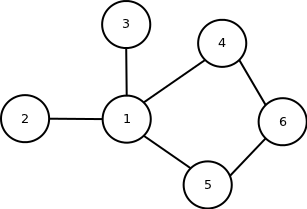
\includegraphics[width=0.4\textwidth]{figures/vizinhos.png}
\caption{A instância de teste triângulo está ligada ao grafo formado pela classe dos círculos e dos losangos, porém não apresenta ligações com os quadrados.}
\label{fig::vizinhos}
\end{figure}

%%%%%%%%%%%%%%%%%%%-------------------------------------------------------%%%%%%%%%%%%%%%%%%%%%%%%%%%%%%%%%%%%%%%%
\subsubsection{Força}
\label{subsubsection::strength}

A métrica \textsc{força(teste,classe)} é uma variação do tamanho da vizinhança de primeira ordem. Quando temos um grafo no qual as arestas têm peso, essa métrica realiza a soma dos pesos das arestas vizinhas ao invés de contar o número das mesmas. O peso de uma aresta, como já dito, é uma forma de representarmos informações importantes em relação aos vértices ligados pela aresta. Em um grafo em que os vértices representam cidades e as arestas representam ligações entre essas cidades, o peso de uma aresta pode significar a distância entre duas cidades, por exemplo. Dessa forma, pode ser mais significativo saber o quão longe (ou perto) uma cidade esta de suas vizinhas do que simplesmente saber o número de vizinhas que a mesma possui.
Destacamos que quando um grafo não possuí pesos nas arestas, atribuímos um peso unitário para todas as arestas, logo a \textsc{força} de um vértice seria igual ao grau de primeira ordem dele.

%%%%%%%%%%%%%%%%%%%-------------------------------------------------------%%%%%%%%%%%%%%%%%%%%%%%%%%%%%%%%%%%%%%%%
\subsubsection{Proximidade}
\label{subsubsection::closeness}

De maneira intuitiva, dizemos que dois objetos estão próximos se eles estão a uma distância arbitrariamente pequena um do outro. Muitas vezes, entretanto, não é fácil estipular o que vem a ser uma distância pequena. 

Em teoria dos grafos, medimos a distância entre os vértices utilizando o algoritmo conhecido como \textit{caminho mínimo}, que caso não leve em consideração o peso das arestas, conta o número mínimo de vértices que necessitamos atravessar para ligar conectar vértices escolhidos em um grafo. A \textsc{Proximidade(teste, classe)} (do inglês, \textit{Closeness}) é uma métrica que estima o quão próximo um vértice $v$ está em relação a todo o grafo usando a média dos caminhos mínimos de $v$ para todos os outros vértices alcançáveis a partir de $v$ (\cite{Beauchamp65}). Dessa forma, podemos medir a importância de um vértice calculando quanto tempo em média é gasto para uma informação se espalhar a partir de um vértice $v$ para todo o resto do grafo. Por fim, são considerados vértices mais ``próximos'' aqueles que minimizam esse tempo.

%%%%%%%%%%%%%%%%%%%-------------------------------------------------------%%%%%%%%%%%%%%%%%%%%%%%%%%%%%%%%%%%%%%%%
\subsubsection{Centralidade}
\label{subsubsection::constraint}
A métrica de centralidade (em inglês, \textit{Betweenness}) \textsc{Centralidade(teste, classe)} se baseia no fato que um vértice é importante em um grafo se ele está no percurso de outros vértices, sendo obrigatoriamente muito visitado. Sendo assim, um vértice tem maior credibilidade se for usado para conectar os vários vértices em um grafo, pertencendo a vários caminhos mínimos.
%Como já dito, o algoritmo do caminho mínimo é o que se utiliza para percorrer da melhor maneira possível uma dada distância em um grafo. 
A métrica \textsc{Centralidade} calcula a importância de um vértice contando quantas vezes aquele vértice participa do caminho mínimo entre quaisquer dois outros vértices do grafo em questão (\cite{Sabidussi66}). Obviamente, um vértice central que está no caminho mínimo de vários outros tem mais acesso a informação que circula pelo grafo que um vértice periférico com poucas ligações.

%%%%%%%%%%%%%%%%%%%-------------------------------------------------------%%%%%%%%%%%%%%%%%%%%%%%%%%%%%%%%%%%%%%%%
\subsubsection{Centralidade do Autovetor.}
\label{subsubsection::eigenvector}

A centralidade do Autovetor (\textsc{Eigen}(teste, classe), do inglês \textit{Eigenvector Centrality}) é uma medida de centralidade que avalia a importância de um vértice em todo o grafo. Ela atribui valores aos vértices baseados nas conexões que os mesmos têm, sendo que um vértice ganhará uma credibilidade maior se estiver conectado a vértices de maior credibilidade. Formalmente, dado que $x_i$ é o valor atribuído ao vértice $i$ e que podemos montar a matriz de adjacência $A$ com os $N$ vértices do grafo, na qual $A_{ij} = 1$ se existe uma aresta entre $i$ e $j$ e $A_{ij}=0$, caso contrário, temos:
\begin{equation}\label{eqn::eigenvector1}
   x_i = \frac{1}{\lambda} \cdot \sum\limits_{j=1}^{N} A_{ij} \cdot x_j
\end{equation}
Que pode ser reescrita utilizando vetores como:
\begin{equation}\label{eqn::eigenvector2}
   X = \frac{1}{\lambda} AX  \;\; \Longleftrightarrow\;\;  AX = \lambda X
\end{equation}
Onde $X$ é dito ser o \textit{autovetor} formado pelos valores de $x_i$ com $0 \leq i \leq N$ e associado ao \textit{autovalor} $\lambda$.  Podem existir muitos valores para $\lambda$ para os quais a Equação~\ref{eqn::eigenvector2} possui solução. Entretanto, se utilizarmos todos os valores do \textit{autovetor} como positivos, teremos o único e maior valor possível para o \textit{autovalor} (\cite{Newman10}). 

%%%%%%%%%%%%%%%%%%%-------------------------------------------------------%%%%%%%%%%%%%%%%%%%%%%%%%%%%%%%%%%%%%%%%
\subsubsection{\textit{Hub} e Autoridade de Kleinberg}
\label{subsubsection::hub}
As métricas conhecidas como \textsc{Hub(teste, classe)} e \textsc{Autoridade(teste, classe)} de Kleinberg são provenientes do trabalho de~\cite{Kleinberg99}. Elas também podem ser apresentadas em conjunto pelo nome de Algoritmo \textit{Hyperlink-Induced Topic Search} (HITS) e por serem predecessoras do \textit{PageRank}.

Em suma, a ideia aqui modelada se baseia no fato de que na \textit{Web}, algumas páginas são conhecidas como \textit{hubs} por não serem especialistas em nenhum assunto específico, mas possuírem ligações para vários outras páginas que são especialistas em seus respectivos assuntos, sendo, portanto, \textit{autoridades} no assunto tratado. Logo, o que temos é que um bom \textit{hub} é representado por uma página (vértice, no grafo que a \textit{Web} representa) que aponta para várias autoridades e uma boa autoridade é aquela apontada por vários \textit{hubs}. Uma página com poucas ligações e com poucas referências não é nem um bom \textit{hub} e nem uma boa autoridade.

%%%%%%%%%%%%%%%%%%%-------------------------------------------------------%%%%%%%%%%%%%%%%%%%%%%%%%%%%%%%%%%%%%%%%
\subsubsection{PageRank}
\label{subsubsection::pagerank}

O algoritmo \textit{PageRank} tem seu nome proveniente do seu criador Lawrence Page (\cite{Page98}). Assim como o algoritmo \textit{HITS}, Seção~\ref{subsubsection::hub}, o \textit{PageRank} se baseia na ideia de ordenar os vértices de um grafo baseado-se nas relações entre eles, sendo que quando mais ``popular'' um vértice é, maior é o seu \textit{PageRank}. Em resumo, temos que
\begin{equation}\label{eqn::pagerank}
PR(teste, classe) = \sum_{v \in Adj(a)} \frac{PR(v, classe)}{L(v)},
\end{equation}
onde $Adj(x)$ é o conjunto dos vizinhos do vértice $x$ e $L(x)$ é o grau de saída de $x$, ou seja, o número de vértices alcançáveis a partir de $x$.

%%%%%%%%%%%%%%%%%%%-------------------------------------------------------%%%%%%%%%%%%%%%%%%%%%%%%%%%%%%%%%%%%%%%%
\subsubsection{Burt's Constraint}
\label{subsubsection::constraint}

O termo capital social é um conceito sociológico abrangente, mas em geral pode-se dizer que está relacionado a relações sociais e consiste na expectativa de benefícios derivados de relações e cooperações entre indivíduos de um grupo e entre os vários grupos existentes na sociedade modelada. Ronald Burt é um sociologista que estudou alguns benefícios que indivíduos podem ter no mercado de trabalho provenientes das relações sociais que mantêm (\cite{Burt92}). Investigando as estruturas de rede do capital social, focando em indivíduos chaves em distintas organizações, ele chegou a conclusão que quem tem boas e diversificadas relações sociais consegue, entre outras coisas, melhores cargos, promoções e salários.  

Outro conceito importante são os buracos estruturais, que podem ser definidos como a falta de acesso entre sub-grafos distintos que compões um mesmo grafo. Burt propôs que vértices que conseguem preenche esses buracos estruturais, unindo vários sub-grafos, são mais importantes que aqueles vértices que estão unidos somente a um mesmo grafo ou os que estão isolados. Esse conceito é usado diretamente para calcular o~\textit{Burt's Constraint} de um vértice. Logo, \textsc{Burt}(teste, classe) é maior se o vértice de teste é capaz de se conectar a mais indivíduos que pertencem a partes não conectadas entre si do grafo modelado pela classe em questão.

%%%%%%%%%%%%%%%%%%%-------------------------------------------------------%%%%%%%%%%%%%%%%%%%%%%%%%%%%%%%%%%%%%%%%
\subsubsection{Bibliographic Coupling}
\label{subsubsection::bibcoup}
%http://igraph.sourceforge.net/doc/html/igraph_bibcoupling.html
\textit{Bibliographic Coupling} é uma métrica introduzida em~\cite{Kessler63} que calcula, para dois trabalhos científicos, o número de referências em comum que ambos possuem. A ideia dessa métrica é que se dois trabalhos apresentam muitas referências em comum, então provavelmente eles abordam o mesmo assunto. Em geral, podemos definir que:
\begin{equation}
\textsc{Bib}(a, b) =  |Adj(a) \cap Adj(b)|,
\end{equation}
onde $Adj(x)$ é o conjunto de vizinhos que o vértice $x$ está conectado. Como estamos interessados em calcular a similaridade de um vértice (exemplo de teste) com uma classe, necessitamos apenas de um valor que defina o quanto aquele vértice se assemelha aos demais. Logo, calculamos o valor do \textit{bibliographic coupling} do exemplo de teste com todos os vértices que ele se conecta:
\begin{equation}
\textsc{BibCoup}(teste, c_j) =  \sum\limits_{v' \in c_j} Bib(teste, v').
\end{equation}

%%%%%%%%%%%%%%%%%%%-------------------------------------------------------%%%%%%%%%%%%%%%%%%%%%%%%%%%%%%%%%%%%%%%%
\subsubsection{Co-Citação}
\label{subsubsection::cocitation}
A métrica co-citação mede, para dois vértices, o número de outros vértices que citam ambos (\cite{Small73}). Assim como a métrica \textit{Bibliographic Coupling}, procuramos atribuir um valor único para um exemplo de teste e, portanto, calculamos o somatório da co-citação entre o teste e todos os vértices presentes no grafo.
%TODO: se eu mudar para um unico grafo de varias classes, tenho que colocar aqui q to levando em consideracao so uma classe por vez.

%%%%%%%%%%%%%%%%%%%-------------------------------------------------------%%%%%%%%%%%%%%%%%%%%%%%%%%%%%%%%%%%%%%%%
\subsubsection{Similaridade de Jaccard}
\label{subsubsection::jaccard}

A similaridade de Jaccard, ver~\cite{Jaccard01}, é uma métrica muito antiga que pode ser definida como o tamanho da interseção de dois conjuntos divididos pela união dos mesmos. Podemos definir a similaridade de Jaccard matematicamente como:
\begin{equation}
\textsc{Jac}(a, b) =  \frac{|Adj(a) \cap Adj(b)|}{|Adj(a) \cup Adj(b)|},
\end{equation}
e da mesma forma que já realizado anteriormente, calculamos o somatório dessa métrica entre o exemplo de teste e todos os vértices do grafo.


%%%%%%%%%%%%%%%%%%%-------------------------------------------------------%%%%%%%%%%%%%%%%%%%%%%%%%%%%%%%%%%%%%%%%
\subsubsection{Similaridade de Dice}
\label{subsubsection::dice}

O coeficiente de similaridade de Dice de dois vértices é duas vezes o número de vizinhos em comum dividido pela soma de graus dos dois vértices, ver~\cite{Dice45}. Matematicamente temos:
\begin{equation}
\textsc{Dice(a,b)} = \frac{2 \cdot | adj(a) \cap adj(b) | }{| a | + | b |},
\end{equation}
onde $adj(x)$ é o conjunto de vértices adjacentes ao vértice $x$. Novamente, calculamos a similaridade de Dice entre o exemplo de teste e todos os vértices do grafo, a fim de termos um único valor que represente a credibilidade do ponto de vista dessa métrica.

%%%%%%%%%%%%%%%%%%%-------------------------------------------------------%%%%%%%%%%%%%%%%%%%%%%%%%%%%%%%%%%%%%%%%
\subsubsection{ Similaridade de Adamic e Adar}
\label{subsubsection::inverselog}

As similaridades de Jaccard e Dice se baseiam no princípio que todos os vértices adjacentes ao vértice que analisamos são igualmente importantes. Entretanto, esse não é sempre o caso.
Inspirados em uma ideia similar ao TDIDF, Seção~\ref{subsubsection::tfidf}, Adamic e Adar propuseram atribuir pesos aos vértices de maneira que um vértice com menos conexões possa ter maior poder discriminativo, ver~\cite{Adamic03}. Dessa forma, a similaridade de Adamic e Adar entre dois vértices é o número de vizinhos que ambos têm em comum, balanceados pelo inverso do logaritmo de seus graus. Ou seja,
\begin{equation}
\textsc{Ad\&Ad(a,b)} =  \sum\limits_{v \in (adj(a)\ \cap\ adj(b))} \frac{1}{ \log(dg(v))},
\end{equation}
onde $dg(g)$ é grau do vértice $v$ e $adj(x)$ é o conjunto de todos os vértices adjacentes de $x$. Como já dito, por fim necessitamos calcular o valor de \textsc{Ad\&Ad(teste, classe)} realizando o somatório da similaridade entre o teste e todos os vértices do grafo da classe em questão.


%\subsubsection{getAvgNearstNeighborDegree(id, className, graphId)}
%\label{subsubsection::avgnearst}
%acho que nao to uando




